\documentclass[tikz,border=4pt]{standalone}
\usetikzlibrary{arrows.meta,calc,positioning}
\begin{document}
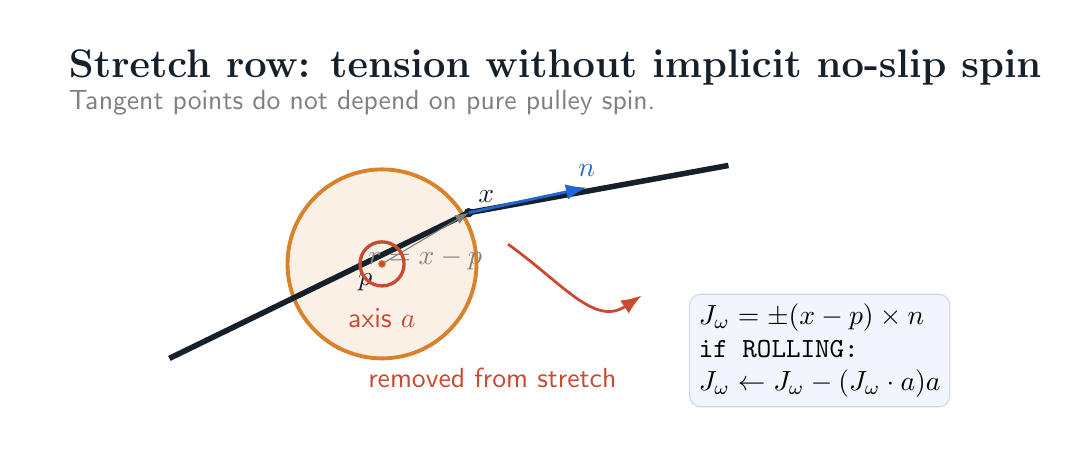
\begin{tikzpicture}[>=Latex, font=\sffamily]
  \definecolor{ink}{HTML}{16202A}
  \definecolor{blue}{HTML}{1F67D2}
  \definecolor{orange}{HTML}{D9822B}
  \definecolor{red}{HTML}{C84B31}
  \draw[fill=white, draw=none] (-0.4,-1.0) rectangle (12.6,4.2);
  \node[anchor=west, font=\bfseries\Large, text=ink] at (0,3.7) {Stretch row: tension without implicit no-slip spin};
  \node[anchor=west, text=gray] at (0,3.25) {Tangent points do not depend on pure pulley spin.};

  \coordinate (p) at (4.1,1.2);
  \coordinate (x) at (5.2,1.85);
  \draw[fill=orange!12, draw=orange, line width=1.4pt] (p) circle (1.2);
  \fill[orange] (p) circle (0.05) node[below left, text=ink] {$p$};
  \fill[ink] (x) circle (0.06) node[above right] {$x$};
  \draw[line width=2pt, color=ink] (1.4,0.0) -- (x) -- (8.5,2.45);
  \draw[->, blue, line width=1pt] (x) -- ++(1.5,0.32) node[above] {$n$};
  \draw[->, gray] (p) -- (x) node[midway, below] {$r=x-p$};
  \draw[red, line width=1.2pt] (p) circle (0.28);
  \fill[red] (p) circle (0.035);
  \node[red, below=0.45cm of p] {axis $a$};
  \draw[->, red, line width=1pt] ($(x)+(0.5,-0.4)$) .. controls +(0.7,-0.5) and +(-0.6,-0.4) .. (7.4,0.8);
  \node[red, anchor=east] at (7.2,-0.25) {removed from stretch};

  \node[draw=blue!25, fill=blue!6, rounded corners, anchor=west, align=left, font=\ttfamily] at (8.0,0.1)
    {$J_\omega=\pm(x-p)\times n$\\if ROLLING:\\$J_\omega\leftarrow J_\omega-(J_\omega\cdot a)a$};
\end{tikzpicture}
\end{document}
